\chapter{Applicazioni astrofisiche}
\label{chap:applicazioni}

\section{Il sistema binario Sgr~A*~-~S2}
\label{sec:sgra}

La terza legge di Keplero permette di determinare la massa di un corpo celeste
se sono noti i parametri orbitali e la massa di un altro corpo con cui
costituisce un sistema binario.

\begin{figure}
  \centering
  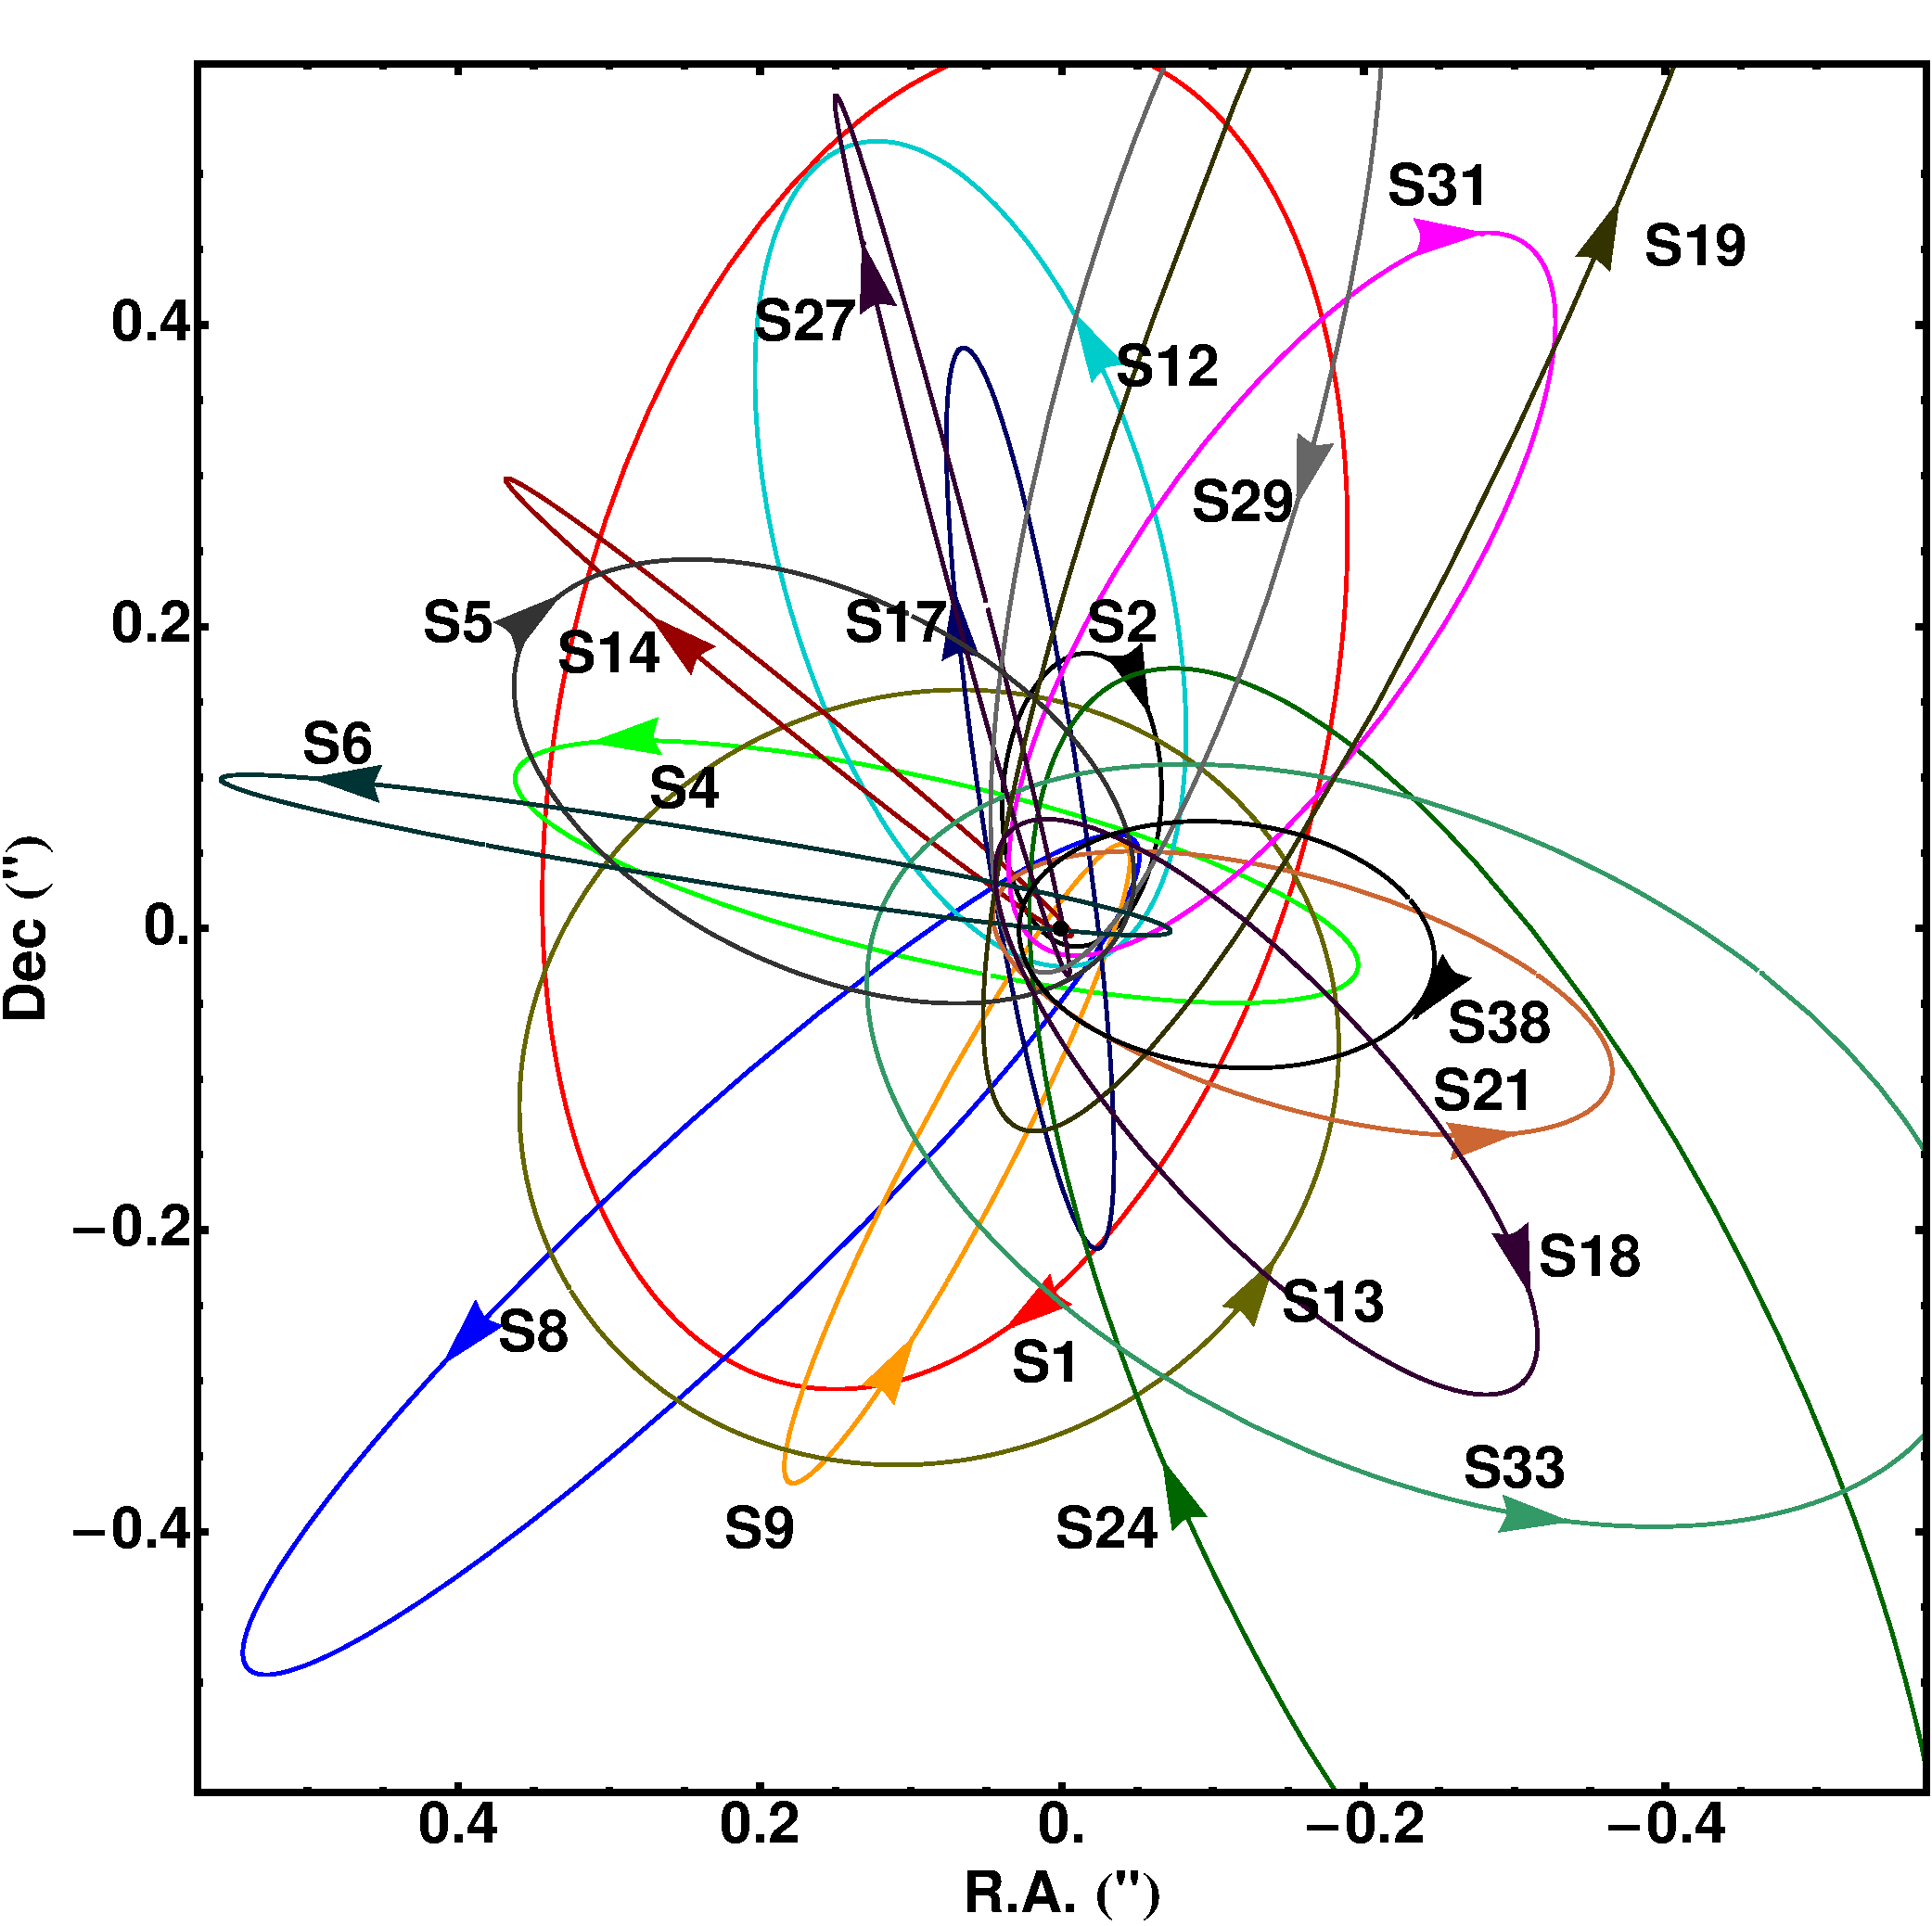
\includegraphics[width=7cm]{Immagini/orbite_sgra}
  \caption[Orbite di alcune delle stelle che intorno al buco nero
  Sgr~A*]{Rappresentazione delle orbite di alcune delle stelle che orbitano
    intorno al buco nero. La figura, tratta da \textcite{2009ApJ...692.1075G}, è
    centrata in Sgr~A*}
  \label{fig:orbite-sgra}
\end{figure}
Si suppone che la regione Sagittarius~A* (Sgr~A*), nel centro della nostra
galassia, sia sede di un buco nero supermassivo, cioè con una massa oltre $10^6$
volte più grande di quella del Sole. Intorno a questo buco nero orbitano
numerose stelle e le orbite di alcune di esse possono essere osservate nella
Figura~\ref{fig:orbite-sgra}. La stella più importante per i nostri scopi è S2
(chiamata a volte S0-2 e di massa circa \SI{15}{\solarmass}), poiché fra le
stelle che orbitano intorno al buco nero è quella che ha il più breve periodo di
rivoluzione, pari a circa $15$ anni, e fra le stelle di questa regione a breve
periodo è la più luminosa, quindi più facile da individuare. Le osservazioni
astronomiche di S2 sono cominciate nel 1992 e da pochi anni ha completato
un'intera rivoluzione a partire da quella data, quindi è una ricca fonte di
informazioni per lo studio del buco nero. L'orbita di S2 intorno al buco nero
può essere considerata con buona approssimazione kepleriana quindi possiamo
utilizzare la~\eqref{eq:terza-legge-keplero} per stimare la massa
$M_\textup{BH}$ del buco nero. \textcite{2008ApJ...689.1044G} hanno studiato il
moto di S2 ricavando i dati riportati nella
Tabella~\ref{tab:parametri-orbitali-S2}.
\begin{table}
  \centering
  \caption[Parametri orbitali della stella S2]{Parametri orbitali della stella
    S2. $R_0$ è la distanza dalla Terra, $P$ è il periodo di rivoluzione, $a$
    è il semiasse maggiore dell'orbita ed $e$ la sua eccentricità,
    $R_\textup{min}$ è la distanza di periapside e $M_{\textup{S}2}$ è la
    massa della stella}
  \label{tab:parametri-orbitali-S2}
  \begin{tabular}{lc}
    \toprule
    Grandezza & Valore \\
    \midrule
    $R_0$ & \SI{7.96}{\kilo\parsec} \\
    $P$ & \SI{15.86}{\year} \\
    $a$ & \SI{126.5}{\milli\arcsecond} \\
    $e$ & $0.8970$ \\
    $R_\textup{min}$ & \SI{0.535}{\milli\parsec} \\
    $M_{\textup{S}2}$ & circa \SI{15}{\solarmass} \\
    \bottomrule
  \end{tabular}
\end{table}
Il semiasse maggiore dell'orbita è espresso in millesimi di arcosecondo, questo
valore può essere convertito in parsec, conoscendo la distanza $R_0$ della Terra
dal corpo, con la seguente relazione
\begin{equation}
  a [\si{\parsec}] = \frac{a [\si{\arcsecond}] \cdot R_0 [\si{\parsec}] \cdot
    \pi}{3600 \cdot 180} = \SI{4.88e-3}{\parsec}.
\end{equation}
Poiché $M_\textup{BH}$ è sicuramente molto più grande di $M_{\textup{S}2}$
possiamo porre $M_\textup{T} \approx M_\textup{BH}$
nella~\ref{eq:terza-legge-keplero} e otteniamo
\begin{equation}
  M_\textup{BH} \approx M_\textup{T} = \frac{4\pi^2a^3}{GP^2} =
  \SI{4.06e6}{\solarmass}.
\end{equation}
In realtà quella calcolata non è esattamente la massa del buco nero ma tutta la
massa che, nel piano dell'orbita di S2, è contenuta nella circonferenza di
raggio $R_\textup{min}$ e centro nel fuoco. Metodi più elaborati per la stima
della massa del buco nero possono essere trovati in
\textcite{2008ApJ...689.1044G} e \textcite{2009ApJ...692.1075G}.

Gli astronomi continuano a studiare il moto di S2 poiché sperano di osservare
delle deviazioni dall'orbita puramente kepleriana previste dalla teoria della
relatività le quali permetterebbero di effettuare una diversa stima della massa
del buco nero.

\section{La funzione di massa. Sistemi binari X}
\label{sec:funzione-massa}

\section{I pianeti extrasolari}
\label{sec:extrasolari}

%%% Local Variables: 
%%% mode: latex
%%% TeX-master: "../tesi"
%%% End: 
